\section{Synthesis of the Cell Envelope}
The subjects of our estimates thus far have been localized to the periphery of
the cell, embedded within the hydrophobic lipid bilayer of the inner membrane.
As outlined in \FIG{energy_scaling}, cells could in principle increase the
expression of the membrane-bound ATP synthases and electron transport chains to
support a larger energy budget across a wide range of cell volumes and membrane
surface areas. This ability, however, is contingent on the ability of the cell
to expand the surface area of the cell by synthesizing new lipids and
peptidoglycan for the cell wall. In this next class of estimates we will
turn our focus to these processes and consider the copy numbers of the relevant
enzymes.

\subsection{Lipid Synthesis}
The cell envelopes of gram negative bacteria (such as \textit{E. coli}) are
composed of an inner and outer phospholipid bilayer membrane separated by a
$\approx 10$ nm periplasmic space (BNID: 100016, \cite{milo2010}). As mentioned
in our discussion of the surface area to volume constraints on energy
production, \textit{E. coli} is a rod-shaped bacterium with a 4:1
length-to-width aspect ratio. At modest growth rates, such as our stopwatch of
5000 s, the total cell surface area is $\approx$ 5 \textmu m$^2$ (BNID: 101792,
\cite{milo2010}). As there are two membranes, each of which composed of two
lipid leaflets, the total membrane area is $\approx 20$\textmu m$^2$, a
remarkable value compared to the $\approx$ 2\textmu m length of the cell.

While this represents the total area of the membrane, this does not mean that it
is composed entirely of lipid molecules. Rather, the dense packing of the
membrane with proteins means that only $\approx$ 40 \% of the membrane area is
occupied by lipids (BNID: 100078, \cite{milo2010}). Using a rule-of-thumb of 0.5
nm$^2$ as the surface area of the typical lipid (BNID: 106993, \cite{milo2010}),
we arrive at an estimate of $\approx$ 2 $\times$ 10$^7$ lipids per cell, an
estimate in close agreement with experimental measurements (BNID: 100071,
102996; \cite{milo2010}).

The membranes of \textit{E. coli} are composed of a variety of different lipids,
each of which is unique in their structures and biosynthetic pathways
\citep{sohlenkamp2016}. With such diversity in biosynthesis, it becomes
difficult to identify which step(s) may be the rate-limiting reactions. This
objective is further complicated by sparsity of \textit{in vivo} kinetic data.
Recently, a combination of stochastic kinetic modeling \citep{ruppe2018} and
\textit{in vitro} kinetic measurements \citep{ranganathan2012, yu2011} have
revealed remarkably slow steps in the fatty acid synthesis pathways which may
serve as the rate limiting reactions. One such step is the removal of hydroxyl
groups from the fatty-acid chain by ACP dehydratase that leads to the formation of
carbon-carbon double bonds. This reaction, catalyzed by proteins FabZ and
FabA in \textit{E. coli} \citep{yu2011}, have been estimated to have kinetic
turnover rates of $\approx$ 1 dehydration per second per enzyme
\citep{ruppe2018}. Combined with this rate, our previous estimates for the
number of lipids to be formed, and a 5000 second division yields an estimate
that the cell requires $\approx$ 4000 ACP dehydratases. This is in
reasonable agreement with the experimentally observed copy numbers of FabZ and
FabA (\FIG{cell_envelope}(A)). Furthermore, we can extend this estimate to
account for the change in membrane surface area as a function of the growth rate
(grey line in \FIG{cell_envelope}(A)), which captures the observed growth rate
dependent expression of these two enzymes.

Despite the slow catalytic rate of FabZ and FabA, we argue that the generation
of fatty acids is not a bottleneck in cell division and is not the key process
responsible for setting the bacterial growth rate. Experimental evidence has
shown that the rate of fatty-acid synthesis can be drastically increased
\textit{in vitro} by increasing the concentration of FabZ \cite{yu2011}.
Stochastic simulations of the complete fatty acid synthesis pathway of
\textit{E. coli} further supports this experimental observation
\cite{ruppe2018}. Thus, if this step was the determining factor in cell
division, increasing growth rate could be as simple as increasing the number of
ACP dehydratases per cell. With a proteome size of $\approx$ 3$\times$10$^6$
proteins, a hypothetical increase in expression from 4000 to 40,000 ACP
dehydratases would result in a $\approx$ 1\% increase in the proteome pool. As
many other  proteins are in much larger abundance than 4000 per cell (as we will
see in the coming sections), it is unlikely that expression of ACP dehydratases
couldn't be increased to facilitate faster growth.


\begin{figure}
    \begin{fullwidth}
    \centering{
        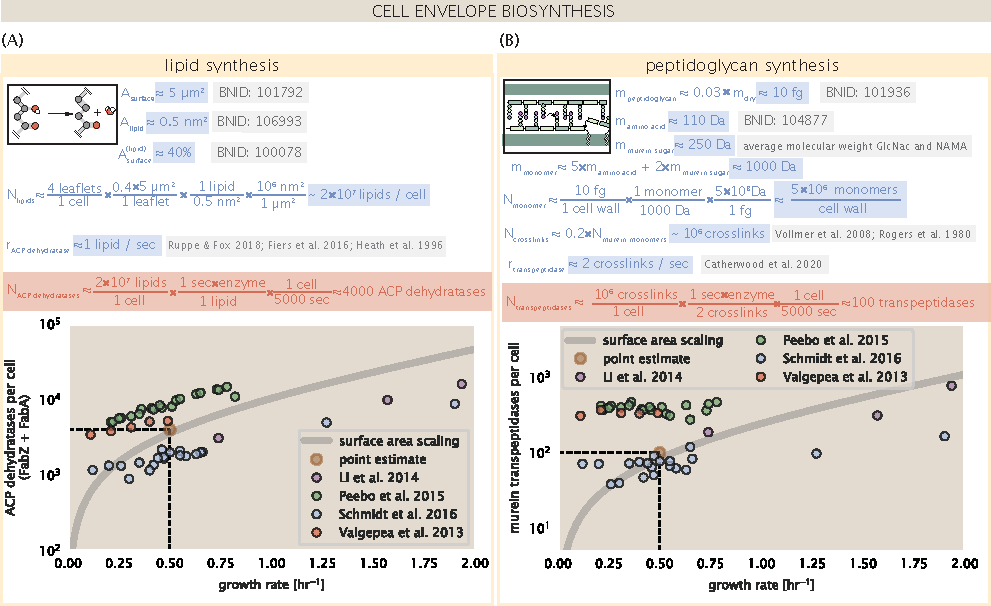
\includegraphics{main_figs/cell_wall_peptidoglycan.pdf}
        \caption{\textbf{Estimation of the key components involved in cell
        envelope biosynthesis.} (A) Top panel shows an estimation for
        the number of ACP dehydratases necessary to form functional
        phospholipids, which is assumed to be a rate-limiting step on lipid synthesis. The rate of ACP dehydratases was inferred from
        experimental measurements via a stochastic kinetic model described in
        \cite{ruppe2018}. Bottom panel shows the experimentally observed complex
        copy numbers using the stoichiometries [FabA]$_2$ and [FabZ]$_2$. (B) An
        estimate for the number of peptidoglycan transpeptidases needed to
        complete maturation of the peptidoglycan. The mass of the murein monomer
        was estimated by approximating each amino acid in the pentapeptide chain
        as having a mass of 110 Da and each sugar in the disaccharide having a
        mass of $\approx$ 250 Da. The \textit{in vivo} rate of transpeptidation
        rein \textit{E. coli} was taken from recent analysis by
        \cite{catherwood2020}. The bottom panel shows experimental measurements
        of the transpeptidase complexes in \textit{E. coli} following the
        stoichiometries [MrcA]$_2$, [MrcB]$_2$, [MrdA]$_1$, and [MrdB]$_1$. Grey
        curves in each plot show the estimated number of complexes needed to
        satisfy the synthesis requirements scaled by the surface area as a
        function of growth rate. We direct the reader to the supplemental
        information for a more detailed discussion of this estimate.
        }
        \label{fig:cell_envelope}
    }
    \end{fullwidth}

\end{figure}


The cell wall is a stiff, covalently linked network composed of PG that surrounds the cell, counteracts turgor pressure, and is a major structural component of the cell envelope.


\subsection{Peptidoglycan Synthesis}
While variation in cell size can vary substantially across growth conditions,
bacterial cells demonstrate exquisite control over their cell shape. The is
primarily due to cell wall, a stiff meshwork of polymerized discaccharides
interspersed with short peptide crosslinks termed the peptidoglycan. The cell
wall is also a vital structural component that conteracts turgor pressure. In
\textit{E. coli}, this enormous peptidoglycan molecule is a few nanometers thick
and resides within the periplasmic space between the inner and outer membrane.
The formation of the peptidoglycan is an intricate process, involving the
bacterial actin homolog MreB \citep{shi2018} along with a variety of
membrane-bound and periplasmic enzymes \citep{morgenstein2015}. The coordinated
action of these components result in a highly-robust polymerized meshwork that
maintains cell shape even in the face of large-scale perturbations and can
restore rod-shaped morphology even after digestion of the peptidoglycan
\citep{harris2018,shi2018}.

In glucose-supported steady-state growth, the peptidoglycan alone comprises
$\approx$ 3\% of the cellular dry mass (BNID: 101936, \cite{milo2010}), making
it the most massive molecule in \textit{E. coli}. The polymerized unit of the
peptidoglycan is a N-acetylglucosamine and N-acetylmuramic acid disaccharide,
the former of which is functionalized with a short pentapeptide. With a mass of
$\approx$ 1000 Da, this unit, which we refer to as a murein monomer, is
polymerized to form long strands in the periplasm which are then attached to
each other via their peptide linkers. Using the aforementioned measurement that
$\approx$ 3\% of the dry mass is peptidoglycan, it can be estimated that the
peptidoglycan is composed of $\approx$ 6$\times$10$^6$ murein monomers.

During growth, peptidoglycan is constantly being broken down to allow insertion
of new murein monomers and cellular expansion. In order to maintain structural
integrity these monomers must be crosslinked into the expanding cell wall,
potentially limiting how quickly new material can be added and we consider this
process as a possible rate-limiting step. In principle,  each one of these
murein monomers can be crosslinked to another glycan strand via the
pentapeptide.  In some species, such as in gram-positive bacterium
\textit{Staphylococcus aureus}, the extent of crosslinking can be large with $>$
90\% of pentapeptides forming a connection between glycan strands. In \textit{E.
coli}, however, a much smaller proportion ($\approx$ 20\%) of the peptides are
crosslinked, resulting in a weaker and more porous cell wall \cite{vollmer2008a,
rogers1980}.  The formation of these crosslinks primarily occur during the
polymerization of the murein monomers and is facilitated by a family of enzymes
called transpeptidases. In \textit{E. coli}, there are four primary
transpeptidases that are involved in lateral and longitudinal extension of the
peptidoglycan. These transpeptidases have only recently been quantitatively
characterized \textit{in vivo} via liquid chromatography mass spectrometry
\citep{catherwood2020}, which revealed a kinetic turnover rate of $\approx 1 -
2$ crosslinking reactions formed per second per enzyme.

Pulling these measurements together permits us to make an estimate that on the
order of $\approx$ 100 transpeptidases are needed for complete maturation of the
peptidoglycan, given a division time of $\approx$ 5000 seconds, a value that is
closely aligned with the experimental observations (\FIG{cell_envelope}(B)). Expanding this
estimate to account for the changing volume of the peptidoglycan as a function
of growth rates (grey line in \FIG{cell_envelope}(B)) also qualitatively captures the observed
dependence in the data, though systematic disagreements between the different
data sets makes the comparison more difficult.

Much as in the case of fatty acid synthesis, we find it unlikely that the
formation of peptidoglycan is a rate limiting step in bacterial cell division.
The estimate we have presented considered only the transpeptidase enzymes that
are involved lateral and longitudinal elongation of the peptidoglycan (proteins
MrdA, MrdB, MrcA, and MrcB). This neglects the presence of other transpeptidases
that are present in the periplasm and also involved in remodeling and maturation
of the peptidoglycan. It is therefore possible that if this was setting the
speed limit for cell division, the simple expression of more
transpeptidases may be sufficient to maintain the structural integrity of the
cell wall.

% Furthermore, it has been shown experimentally that, while critical for cell
% wall formation, there are components needed beyond the transpeptidases to
% maintain cell shape and permit cell division. For example, the bacterial actin
% homolog MreB polymerizes laterally along the inner membrane and facilitates the
% longitudinal expansion of the peptidoglycan. Inhibition of MreB through the
% addition of small molecule inhibitors results in loss of the cell shape, but formation
% of the peptidoglycan is otherwise not significantly hindered \cite{shi2018}. This suggests
% that in considering the development of the cell envelope, proper assembly may
% be a more important property to consider beyond synthesis of the appropriate
% number of glycan polymers.
